% !TEX encoding = UTF-8
% !TEX TS-program = pdflatex
% !TEX root = ../tesi.tex

%**************************************************************
\chapter{Progettazione}
\label{cap:progettazione}
%**************************************************************

\intro{Questo capitolo illustra le motivazioni alla base delle scelte progettuali adottate nello sviluppo del prototipo da me realizzato durante l'esperienza di stage.}\\ %TODO oppure illustra lo stato dell'applicazione

\section{Architettura preesistente}
Trattandosi di una reimplementazione di una funzionalità preesistente, il primo ostacolo è stato quello di capire come dovesse integrarsi con il resto dell'architettura con cui avrei dovuto interagire, per questo motivo la prima settimana di stage è stata dedicata quasi esclusivamente alla conoscenza dell'ambiente e delle componenti. \\
\subsection{Visione generale}

\begin{figure}[h]
	\centering
	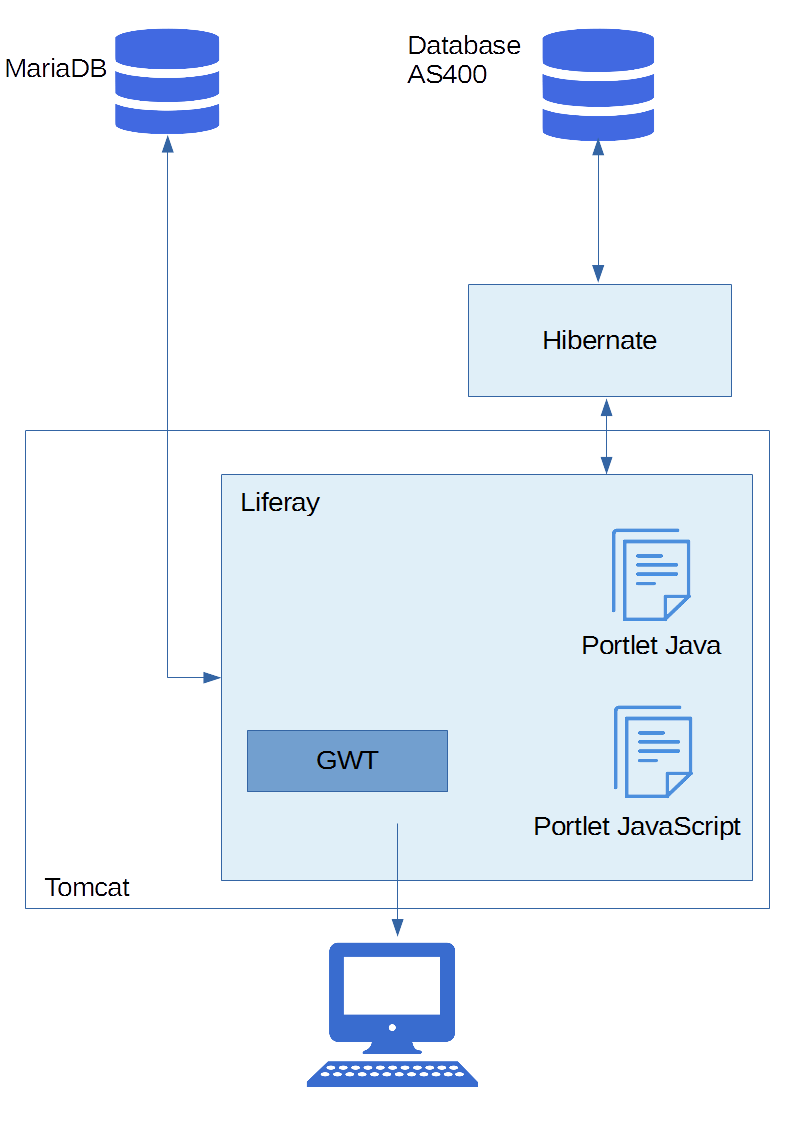
\includegraphics[height = 15 cm]{schema-generale}
	\caption{Schema generale di interconnessione tra le componenti}
	\label{schema-generale}
\end{figure}
la figura \ref{schema-generale} illustra, ad alto livello, le relazioni che intercorrono tra le varie tecnologie utilizzate dal software JGalileo CRM.\\
Partendo dalle basi di dati fino ad arrivare all'interfaccia utente, l'architettura del sistema si snoda in questo modo:\\
Entrambe le basi di dati, sia quella contenuta nel database del sistema operativo AS400 che quella contenuta sul server, si interfacciano con il Framework Hibernate per creare delle classi, equivalenti alle tabelle del database, con cui permettere l'interazione.\\
L'interazione con le entità di Hibernate avviene per mezzo di Liferay, che si occupa anche della gestione degli accessi degli utenti alla pagina, introducendo il concetto di Single Sing On, e della corretta visualizzazione delle portlet all'interno delle pagine del portale. Queste posso essere scritte in AngularJS, come ad esempio le portlet scritte da me, oppure in Java e successivamente tradotte in JavaScript tramite i servizi offerti da GWT.\\
Le azioni dell'utente vengono gestite poi da Liferay, che si occupa anche del routing tra le varie pagine del portale. Nel caso ci fossero dei dati da salvare, come nel aso dell'inserimento di un nuovo lead, vengono lanciati dei servizi REST che andranno ad interfacciarsi con le entità gestite da Hibernate, il quale garantisce la persistenza dei dati.
	